
% This LaTeX was auto-generated from MATLAB code.
% To make changes, update the MATLAB code and republish this document.

\documentclass{article}
\usepackage{graphicx}
\usepackage{color}

\sloppy
\definecolor{lightgray}{gray}{0.5}
\setlength{\parindent}{0pt}

\begin{document}

    
    

\section*{13. Equispaced points, Runge phenomenon}

\begin{verbatim}
ATAPformats
\end{verbatim}
\begin{par}
So far in this book, we have considered three good methods for approximating functions by polynomials: Chebyshev interpolation, Chebyshev projection, and best approximation.  Now we shall look at a catastrophically bad method!---interpolation in equally spaced points. This procedure is so unreliable that for generations, it has tainted people's views of the whole subject of polynomial interpolation. The mathematical tools we will need to understand what is going on are the Hermite integral formula and potential theory, as discussed in the last two chapters.
\end{par} \vspace{1em}
\begin{par}
As mentioned in Chapter 5, polynomial interpolation was an established tool by the 19th century. The question of whether or not polynomial interpolants would converge to an underlying function as $n\to \infty$ was not given much attention.  Presumably many mathematicians would have supposed that if the function was analytic, the answer would be yes.  In 1884 and 1896, $\hbox{M\'eray}$ published a pair of papers in which he identified the fact that certain interpolation schemes do not converge $\hbox{[M\'eray}$ 1884 \& 1896].  In the first paper he writes,
\end{par} \vspace{1em}
\begin{par}

\em It is rather astonishing that practical applications have not yet
turned up any cases in which the interpolation is illusory.\footnote{``Il
est assez \'etonnant que les hasards de la pratique n'aient encore fait
conna\^itre aucun cas dans lequel l'interpolation soit illusoire.'' By
illusory, M\'eray means nonconvergent.}

\end{par} \vspace{1em}
\begin{par}

M\'eray's derivations had the key idea of making use of the
Hermite integral formula.  However, the examples he devised were rather
contrived, and his idio\-syncratically written papers had little impact. It
was Runge in 1901 who made the possibility of divergence famous by
showing that divergence of interpolants occurs in general even for
equispaced points in an real interval and evaluation points in the
interior of that interval [Runge 1901].

\end{par} \vspace{1em}
\begin{par}

Runge illustrated his discovery with an example that has become known as
the {\em Runge function}: $1/(1+x^2)$ on $[-5,5]$, or equivalently,
$1/(1+25x^2)$ on $[-1,1]$:

\end{par} \vspace{1em}
\begin{par}
 \vskip -2em 
\end{par} \vspace{1em}
\begin{verbatim}
x = chebfun('x'); f = 1./(1+25*x.^2);
\end{verbatim}
\begin{par}
We already know from Chapter 8 that there is nothing wrong with this function for polynomial interpolation in Chebyshev points: $f$ is analytic, and the polynomial interpolants converge geometrically.  Now, however, let us follow Runge and look at interpolants in equally spaced points, which we can compute using the Chebfun overload of Matlab's \texttt{interp1} command.
\end{par} \vspace{1em}
\begin{par}
Here is what we get with 8 points:
\end{par} \vspace{1em}
\begin{par}
 \vskip -2em 
\end{par} \vspace{1em}
\begin{verbatim}
s = linspace(-1,1,8); p = interp1(s,f,domain(-1,1));
hold off, plot(f), hold on, plot(p,'r'), grid on
plot(s,p(s),'.r'), axis([-1 1 -1 3]), FS = 'fontsize';
title('Equispaced interpolation of Runge function, 8 points',FS,9)
\end{verbatim}

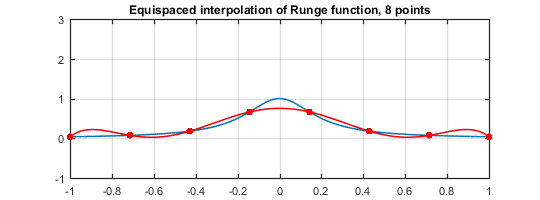
\includegraphics [width=4in]{chap13_01.png}
\begin{par}
 \vskip 1pt 
\end{par} \vspace{1em}
\begin{par}
Here is the result for 16 points:
\end{par} \vspace{1em}
\begin{par}
 \vskip -2em 
\end{par} \vspace{1em}
\begin{verbatim}
s = linspace(-1,1,16); p = interp1(s,f,domain(-1,1));
hold off, plot(f), hold on, plot(p,'r'), grid on
plot(s,p(s),'.r'), axis([-1 1 -1 3])
title('Equispaced interpolation of Runge function, 16 points',FS,9)
\end{verbatim}

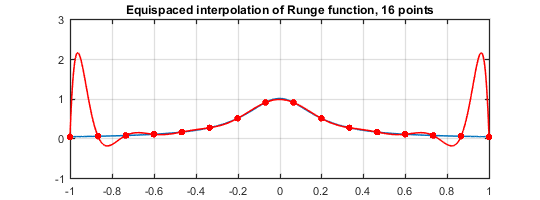
\includegraphics [width=4in]{chap13_02.png}
\begin{par}
 \vskip 1pt 
\end{par} \vspace{1em}
\begin{par}
Is this going to converge as $n\to\infty$? Things look pretty good in the middle, but not so good at the edges.  Here is the result for 20 points:
\end{par} \vspace{1em}
\begin{par}
 \vskip -2em 
\end{par} \vspace{1em}
\begin{verbatim}
s = linspace(-1,1,20); p = interp1(s,f,domain(-1,1));
hold off, plot(f), hold on, plot(p,'r'), grid on
plot(s,p(s),'.r'), axis([-1 1 -1 3])
title('Equispaced interpolation of Runge function, 20 points',FS,9)
\end{verbatim}

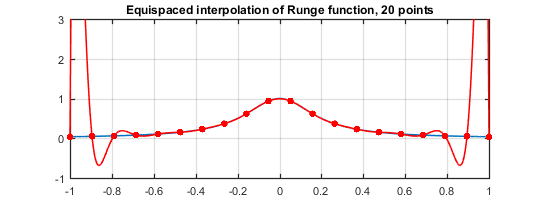
\includegraphics [width=4in]{chap13_03.png}
\begin{par}
 \vskip 1pt 
\end{par} \vspace{1em}
\begin{par}
What is happening is exponential convergence in the middle of the interval but exponential divergence near the ends. The next figure shows the maximum error over $[-1,1]$ as a function of the number of points.  We get a hint of convergence at first, but after $n=10$, things just get worse. Note the log scale.
\end{par} \vspace{1em}
\begin{par}
 \vskip -2em 
\end{par} \vspace{1em}
\begin{verbatim}
ee = []; nn = 2:2:50;
for np = nn
  s = linspace(-1,1,np); p = interp1(s,f,domain(-1,1));
  ee = [ee norm(f-p,inf)];
end
hold off, semilogy(nn,ee,'.-'), grid on, axis([0 50 5e-2 2e6])
xlabel n+1, title('Divergence as n+1 -> \infty',FS,9)
\end{verbatim}

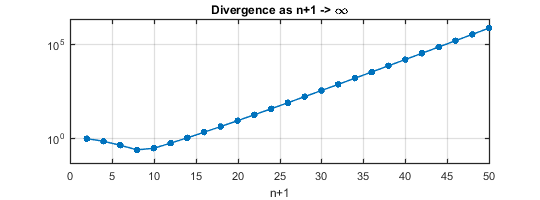
\includegraphics [width=4in]{chap13_04.png}
\begin{par}
 \vskip 1pt 
\end{par} \vspace{1em}
\begin{par}
By now the reader may have suspected that what is going wrong here can be understood by looking at potentials, as in the last two chapters. Here is an adaptation of a code segment from Chapter 11 to plot equipotential curves for $n+1 = 8$ and $20$.
\end{par} \vspace{1em}
\begin{par}
 \vspace{-2em} 
\end{par} \vspace{1em}
\begin{verbatim}
d = domain(-1.5,1.5);
xgrid = -1.5:.02:1.5; ygrid = -1:.02:1;
[xx,yy] = meshgrid(xgrid,ygrid); zz = xx+1i*yy;
for np = [8 20]
  xj = linspace(-1,1,np);
  ell = poly(xj,d);
  hold off, plot(xj,ell(xj),'.k','markersize',8)
  hold on, ylim([-1.2 1.2]), axis equal
  ellzz = ell(zz);
  levels = ((1.25:.25:3)/exp(1)).^np;
  contour(xx,yy,abs(ellzz),levels,'k')
  title(['Level curves of |l(x)| for '...
    int2str(np) ' equispaced points'],FS,9)
  snapnow
end
\end{verbatim}

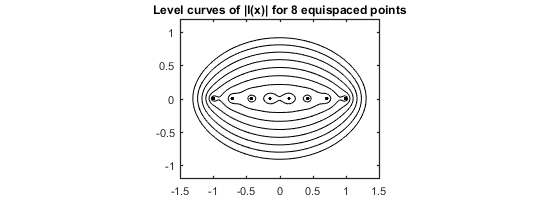
\includegraphics [width=4in]{chap13_05.png}

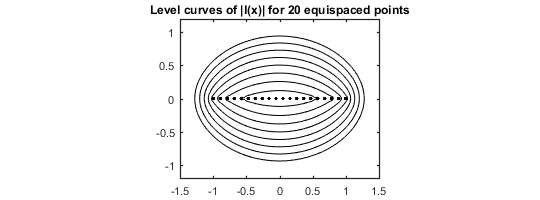
\includegraphics [width=4in]{chap13_06.png}
\begin{par}
 \vspace{1pt} 
\end{par} \vspace{1em}
\begin{par}
What we see here is that $[-1,1]$ is very far from being a level curve for equispaced interpolation points. From the last two chapters, we expect serious consequences of this irregularity.  In the second plot just shown, for example, it is the fourth curve (from inside out) that approximately touches the endpoints $\pm 1$.  For Theorem 11.1 to be of any use in such a landscape, $f$ will have to be analytic in a region larger than the ``football'' enclosed by that curve.  Analyticity on $[-1,1]$ is not enough for convergence; we will need analyticity in a much bigger region of the complex plane. This is what Runge discovered in 1901.
\end{par} \vspace{1em}
\begin{par}
Following the method of the last chapter, we now consider the limit $n\to\infty$, where the distribution of interpolation points approaches the constant measure (12.9), $$ \mu(\tau) = {1\over 2} . \eqno (13.1) $$ The potential (12.7) associated with this measure is $$ u(s) = -1 + {1\over 2}\hbox{Re} \left[(s+1)\log(s+1)-(s-1)\log(s-1)\right]. \eqno (13.2) $$ Here is a code that plots just one level curve of this potential, the one passing through $\pm 1$, where the value of the potential is $-1 + \log 2$.
\end{par} \vspace{1em}
\begin{par}
 \vskip -2em 
\end{par} \vspace{1em}
\begin{verbatim}
x1 = -1.65:.02:1.65; y1 = -0.7:.02:0.7;
[xx,yy] = meshgrid(x1,y1); ss = xx+1i*yy;
u = @(s) -1 + 0.5*real((s+1).*log(s+1)-(s-1).*log(s-1));
hold off
contour(x1,y1,u(ss),(-1+log(2))*[1 1],'k','linewidth',1.4)
set(gca,'xtick',-2:.5:2,'ytick',-.5:.5:.5), grid on
ylim([-.9 .9]), axis equal
hold on, plot(.5255i,'.k')
text(0.05,.63,'0.52552491457i')
title(['Runge region for equispaced interpolation ' ...
       'in the limit n -> \infty'],FS,9)
\end{verbatim}

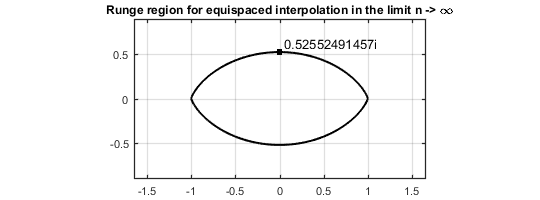
\includegraphics [width=4in]{chap13_07.png}
\begin{par}
 \vskip 1pt 
\end{par} \vspace{1em}
\begin{par}
For the interpolants to a function $f$ in equispaced nodes to converge as $n\to\infty$ for all $x\in[-1,1]$, $f$ must be analytic, not just on $[-1,1]$, but throughout this \textit{Runge region,} which crosses the real axis at $\pm 1$ and the imaginary axis at $\pm 0.52552491457\dots i.$  Runge reports this number correctly to 4 digits, and writes
\end{par} \vspace{1em}
\begin{par}

\em The curve has somewhat the shape of an ellipse.  At the ends of the
long axis, however, our curve is more pointed than an
ellipse.\footnote{``Die Kurve$\dots$ hat etwa die Gestalt einer
Ellipse$\dots.$  An den Enden der grossen Achse ist unsere Kurve aber
spitzer als eine Ellipse.''} 
\end{par} \vspace{1em}
\begin{par}
Here are the values of (13.2) at the endpoints and the middle: $$ u(\pm 1) = -1 + \log 2, \quad u(0) = -1, $$ and thus $$ \exp( u(\pm 1))= {2\over e}, \quad \exp(u(0)) = {1\over e}. $$ These numbers indicate that in the limit $n\to\infty$, the endpoints of an equispaced grid in $[-1,1]$ lie at an average distance $2/e$ from the other grid points, in the geometric mean sense, whereas the midpoint lies at an average distance of just $1/e$. As emphasized in the last chapter, notably in equation (12.6), the effect of such a discrepancy grows exponentially with $n$.
\end{par} \vspace{1em}
\begin{par}
Here are some examples. Equispaced interpolation will converge throughout $[-1,1]$ for $f(x) = \exp(-x^2)$, which is analytic everywhere, and for $f(x) = (1+x^2)^{-1}$, which has poles at $\pm i$.  On the other hand it will not converge for $f(x) = (1+16x^2)^{-1}$, which has poles at $\pm i/4$. It will converge slowly for $f(x) = (1+(x/0.53)^2)^{-1}$, and diverge slowly for $f(x) = (1+(x/0.52)^2)^{-1}$ (Exercise 13.3).
\end{par} \vspace{1em}
\begin{par}
The worst-case rate of divergence is $2^n$, and this rate will always appear if $f$ is not analytic on $[-1,1]$. To be precise, for such a function the errors will be of size $O(2^n)$ as $n\to\infty$ but not of size $O(C^n)$ for any $C<2$.  Here, for example, we take $f$ to be a hat function, with just one derivative of bounded variation. The dots show errors in Chebyshev interpolation, converging at the rate $O(n^{-1})$ in keeping with Theorem 7.2, and the crosses show errors in equispaced interpolation, with a dashed line parallel to $2^n$ for comparison.
\end{par} \vspace{1em}
\begin{par}
 \vskip -2em 
\end{par} \vspace{1em}
\begin{verbatim}
f = max(0,1-2*abs(x));
eequi = []; echeb = []; nn = 2:2:60;
for n = nn
  s = linspace(-1,1,n+1);
  pequi = interp1(s,f,domain(-1,1)); eequi = [eequi norm(f-pequi,inf)];
  pcheb = chebfun(f,n+1); echeb = [echeb norm(f-pcheb,inf)];
end
hold off, semilogy(nn,2.^(nn-12),'--r')
hold on, axis([0 60 1e-4 1e14]), grid on
semilogy(nn,eequi,'x-r','markersize',8), semilogy(nn,echeb,'.-b')
text(47,3e6,'equispaced','color','r')
text(41,0.8,'Chebyshev','color','b')
text(32,4e8,'C 2^n','fontsize',12,'color','r')
xlabel np, ylabel Error, title('Chebyshev vs. equispaced points',FS,9)
\end{verbatim}

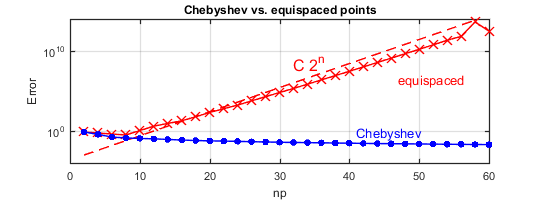
\includegraphics [width=4in]{chap13_08.png}
\begin{par}
 \vskip 1pt 
\end{par} \vspace{1em}
\begin{par}
All of the above remarks about equispaced interpolation concern the ideal mathematics of the problem.  On a computer in floating point arithmetic, however, a further complication arises: even if convergence ought to take place in theory, rounding errors will be amplified by $O(2^n)$, causing divergence in practice. Here, for example, are the errors in equispaced and Chebyshev interpolation of the entire function $\exp(x)$:
\end{par} \vspace{1em}
\begin{par}
 \vskip -2em 
\end{par} \vspace{1em}
\begin{verbatim}
f = exp(x);
eequi = []; echeb = []; nn = 2:2:80;
for n = nn
  s = linspace(-1,1,n+1);
  pequi = interp1(s,f,domain(-1,1)); eequi = [eequi norm(f-pequi,inf)];
  pcheb = chebfun(f,n+1); echeb = [echeb norm(f-pcheb,inf)];
end
hold off, semilogy(nn,2.^(nn-50),'--r')
hold on, axis([0 80 1e-17 1e4]), grid on
semilogy(nn,eequi,'x-r','markersize',8), semilogy(nn,echeb,'.-b')
text(22,6e-6,'C 2^n','fontsize',12,'color','r')
text(42,3e-7,'equispaced','color','r')
text(51,6e-14,'Chebyshev','color','b')
xlabel np, ylabel Error, title('The effect of rounding errors',FS,9)
\end{verbatim}

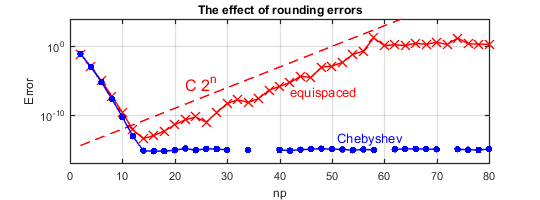
\includegraphics [width=4in]{chap13_09.png}
\begin{par}
 \vskip 1pt 
\end{par} \vspace{1em}
\begin{par}
In exact arithmetic we would see convergence for both sets of points, but on the computer the divergence for equispaced points sets in early.  The rate is cleanly $O(2^n)$ until we reach $O(1)$. Notice that the line of crosses, if extended backward to $n=0$, meets the $y$ axis at approximately $10^{-18}$, i.e., a digit or two below machine precision.
\end{par} \vspace{1em}
\begin{par}
The $2^n$ divergence of equispaced polynomial interpolants is a fascinating subject, and we must remind ourselves that one should only go into so much detail in analyzing a method that should never be used! But perhaps we should qualify that ``never'' in one respect. As Runge himself emphasized, though interpolants in equispaced points do not converge on the whole interval of interpolation, they may still do very well near the middle.  In the numerical solution of differential equations, for example, higher order centered difference formulas are successfully used based on 5 or 7 equally spaced grid points.  A less happy example would be Newton--Cotes quadrature formulas, based on polynomial interpolation in equally spaced points, where the $O(2^n)$ effect is unavoidable and causes serious problems for larger $n$ and divergence as $n\to\infty$, as first proved by $\hbox{P\'olya}$ [1933]. We shall discuss quadrature in Chapter 19.
\end{par} \vspace{1em}
\begin{par}
We close this chapter with an observation that highlights the fundamental nature of the Runge phenomenon and its associated mathematics. Suppose you want to persuade somebody that it is important to know something about complex variables, even for dealing with real functions.  I still remember the argument my calculus teacher explained to me: to understand why the Taylor series for $1/(1+x^2)$ only converges for $-1 < x < 1$, you need to know that Taylor series converge within disks in the complex plane, and this function has poles at $\pm i$.
\end{par} \vspace{1em}
\begin{par}
Runge's observation is precisely a generalization of this fact to interpolation points equispaced in an interval rather than all at $x=0$. The convergence or divergence of polynomial interpolants to a function $f$ again depends on whether $f$ is analytic in a certain region; the change is that the region is now not a disk, but elongated. Even the phenomenon of divergence in floating-point arithmetic for functions whose interpolants ``ought'' to converge is a generalization of familiar facts from real arithmetic.  Just try to evaluate $\exp(x)$ on a computer for $x=-20$ using the Taylor series!
\end{par} \vspace{1em}
\begin{par}

\begin{displaymath}
\framebox[4.7in][c]{\parbox{4.5in}{\vspace{2pt}\sl
{\sc Summary of Chapter 13.}
Polynomial interpolation in equispaced points is exponentially
ill-conditioned: the interpolant $p_n$ may have oscillations near the
edge of the interval nearly $\kern .7pt 2^n$ times larger than the function $f$
being interpolated, even if $f$ is analytic.  In particular, even if $f$
is analytic and the interpolant is computed exactly without rounding
errors, $p_n$ need not converge to $f$ as $n\to\infty$.\vspace{2pt}}}
\end{displaymath}

\end{par} \vspace{1em}
\begin{par}
 \smallskip \parskip=2pt\small
{\bf Exercise 13.1.  Three examples.}
Draw plots comparing accuracy of equispaced
and Chebyshev interpolants as functions of $n$ for
$\exp(x^2)$, $\exp(-x^2)$, $\exp(-1/x^2)$.
\par
{\bf Exercise 13.2.  Computing geometric means in Chebfun.}
(a) What output is produced by the program below?  (b) Why?
\par\verb|x = chebfun('x',[0 1]);|
\hfill\break\verb|f = chebfun(@(y) prod(abs(x-1i*y)),[0.1 1],'vectorize');|
\hfill\break\verb|roots(f-2/exp(1))|
\par
{\bf Exercise 13.3. Borderline convergence.}
The claim was made in the text that equi\-spaced
polynomial interpolants on $[-1,1]$ converge
for $f(x) = (1+(x/0.53)^2)^{-1}$ and diverge for
$f(x) = (1+(x/0.52)^2)^{-1}$.  Can you observe this difference
numerically?  Run appropriate experiments and discuss the results.
\par
{\bf Exercise 13.4.  Approaching the sinc function.}
The sinc function is defined for all $x$ by $S(x) = \sin(\pi x)/(\pi x)$
(and $S(0) = 1$).
For any $n\ge 1$, an approximation to $S$ is given by
$$ S_n = \prod_{k=1}^n (1-x^2/k^2).  $$
Construct $S_{20}$ in Chebfun on the interval $[-20,20]$ and
compare it with $S$.  On what interval around $x=0$ do you
find $|S_{20}(x)-S(x)| < 0.1$?  (It can be shown that for
every $x$, $\lim_{n\to \infty} S_n(x) = S(x)$.)
\par
{\bf Exercise 13.5.  Barycentric weights and ill-conditioning.}
(a) Suppose a function is interpolated by a polynomial in $n+1$
equispaced points in $[-1,1]$, with $n$ even.  From the result of Exercise 5.6,
derive a formula for the ratio of the barycentric weights at
the midpoint $x=0$ and the endpoint $x=1$.
(b) With reference to the barycentric formula (5.11), explain what
this implies about sensitivity of these polynomial interpolants
to perturbations in the data at $x=0$.
\par 
\end{par} \vspace{1em}



\end{document}
    
